\documentclass[%
	corpo=11pt,
    twoside,
    stile=classica,
    oldstyle,
    tipotesi=custom,
    greek,
    evenboxes,
]{toptesi}
%%%%%%%%%%%%%%%%%%%%%%%%%%%%%%%%%%%%%%%%%%%%%%%%%%%%

\usepackage[utf8]{inputenc}
\usepackage[T1]{fontenc}
\usepackage{lmodern}

\usepackage{hyperref}
\hypersetup{%
    pdfpagemode={UseOutlines},
    bookmarksopen,
    pdfstartview={FitH},
    colorlinks,
    linkcolor={blue},
    citecolor={blue},
    urlcolor={blue}
  }

%%%%%%% use PDFLATEX 

\usepackage{lipsum} %to insert random text

\usepackage{geometry} %for the margins
\newcommand\fillin[1][5cm]{\makebox[#1]{\dotfill}} %for the dotted line in the frontispiace

\usepackage{dcolumn}
\newcolumntype{d}{D{.}{.}{-1} } %to vetical align numbers in tables, along the decimal dot

\usepackage{amsmath}

\usepackage{natbib} % for the bibliography
\bibliographystyle{plainnat}


%%%%%%% Local definitions
\newtheorem{osservazione}{Osservazione}% Standard LaTeX
\newtheorem{observation}{Observation}% Standard LaTeX


%%%%%%% Custom fonts for title page
\newcommand\customfont[1]{{\usefont{T1}{Poppins-Regular}{m}{n} #1 }}

%%%%%%%%%%%%%%%%%%%%%%%%%%%%%%%%%%%%%%%%%%%%%%%%
%%%%%%%%%%%%%%%%%%%%%%%%%%%%%%%%%%%%%%%%%%%%%%%%



\begin{document}\errorcontextlines=9
\english

\begin{titlepage}
\newgeometry{left=1cm,right=1cm,top=3cm,bottom=3.5cm}  %specific margins for this page

\begin{center}

{\huge POLITECNICO DI TORINO}\\[1.5cm]
\textbf{Corso di Laurea Magistrale\\in Ingegneria Informatica}\\[3cm]
%\textbf{Corso di Laurea Magistrale\\in Ingegneria Matematica}\\[3cm]

{\Large Tesi di Laurea}\\[1cm]
%{\Large Tesi di Laurea Magistrale}\\[0.5cm]
\textbf{\LARGE Edge-to-Cloud Multi-Cluster Orchestration for Smart Grid Monitoring Services  }\\[2cm]

\includegraphics[width=0.2\textwidth]{./Pictures/logo_polito_2021.jpg}
\vspace{4cm}

\customfont{hello world!}

\begin{minipage}{0.85\textwidth}
\begin{flushleft}\large
\textbf{Relatori} \hfill \textbf{Candidato}\\
prof. Fulvio Risso \hfill Riccardo Medina\\
ing. Stefano Galantino \\
\textit{firma dei relatori} \hfill \textit{firma del candidato}\\[0.35cm]
\fillin\ \hfill \\
\fillin\ \hfill \fillin
\end{flushleft}
\end{minipage}

\vfill

Anno Accademico 2023-2024
\end{center}

\restoregeometry %restor default margins 

\end{titlepage} %the frontispiece

%%%%%%% Dedication
\ifclassica%
{\begin{dedica}
    A mio padre

    \textdagger\ A mio nonno Pino
\end{dedica}
%%%%%%% 

\sommario%summary
%Here goes the abstrat of your thesis
La pressione barometrica di Giove viene misurata mediante un metodo originale  messo a punto dai candidati, che si basa sul rilevamento telescopico della pressione.

%%%%%%%%%%%%%%%%%%%%%%%%%%%%%%%%%%%%%%%%%%%%%%%%
%%%%%%%%%%%%%%%%%%%%%%%%%%%%%%%%%%%%%%%%%%%%%%%%

\ringraziamenti%acknowledgements
%Acknowledge the people you love and/or work with
I candidati ringraziano vivamente il Granduca di Toscana per i mezzi messi loro a disposizione, ed il signor Von Braun, assistente del prof.~Albert Einstein, per le informazioni riservate che egli ha gentilmente fornito loro, e per le utili discussioni che hanno permesso ai candidati di evitare di riscoprire l'acqua calda.

%%%%%%%%%%%%%%%%%%%%%%%%%%%%%%%%%%%%%%%%%%%%%%%%
%%%%%%%%%%%%%%%%%%%%%%%%%%%%%%%%%%%%%%%%%%%%%%%%

\tablespagetrue\figurespagetrue%to include the list of tables
%and the list of figures - yuo can comment these commands

\indici%table of content
%It automatically generated

%%%%%%%%%%%%%%%%%%%%%%%%%%%%%%%%%%%%%%%%%%%%%%%%
%%%%%%%%%%%%%%%%%%%%%%%%%%%%%%%%%%%%%%%%%%%%%%%%

\mainmatter


\chapter{Introduzione generale}

\section{Principi generali}
Il problema della determinazione della pressione barometrica dell'atmosfera di Giove non ha ricevuto finora una soluzione soddisfacente, per l'elementare motivo che il pianeta suddetto si trova ad una distanza tale che i mezzi attuali non consentono di eseguire una misura diretta.

Conoscendo per\`o con grande precisione le orbite dei satelliti principali di Giove, e segnatamente le orbite dei satelliti medicei, \`e possibile eseguire delle misure indirette, che fanno ricorso alla nota formula \cite{gal}:
\begin{equation} \label{eq:eq1}
\Phi = K\frac{\Xi^2 +\Psi_\mathrm{max}}{1+\gei\Omega}\ .
\end{equation}

In \eqref{eq:eq1} le varie grandezze hanno i seguenti significati:
\begin{enumerate}
\item $\Phi$ angolo di rivoluzione del satellite in radianti se $K=1$, in gradi se $K=180/\pi$;
\item $\Xi$ eccentricit\`a dell'orbita del satellite; questa \`e una grandezza priva di dimensioni;
\item $\Psi_\mathrm{max}$ rapporto fra il semiasse maggiore ed il semiasse minore dell'orbita del satellite, nelle condizioni di massima eccentricit\`a;
\item $\Omega$ velocit\`a istantanea di rotazione; 
\end{enumerate}

Le grandezze in gioco sono evidenziate nella Figura \ref{fig:figura}.
\begin{figure}[htb]\centering
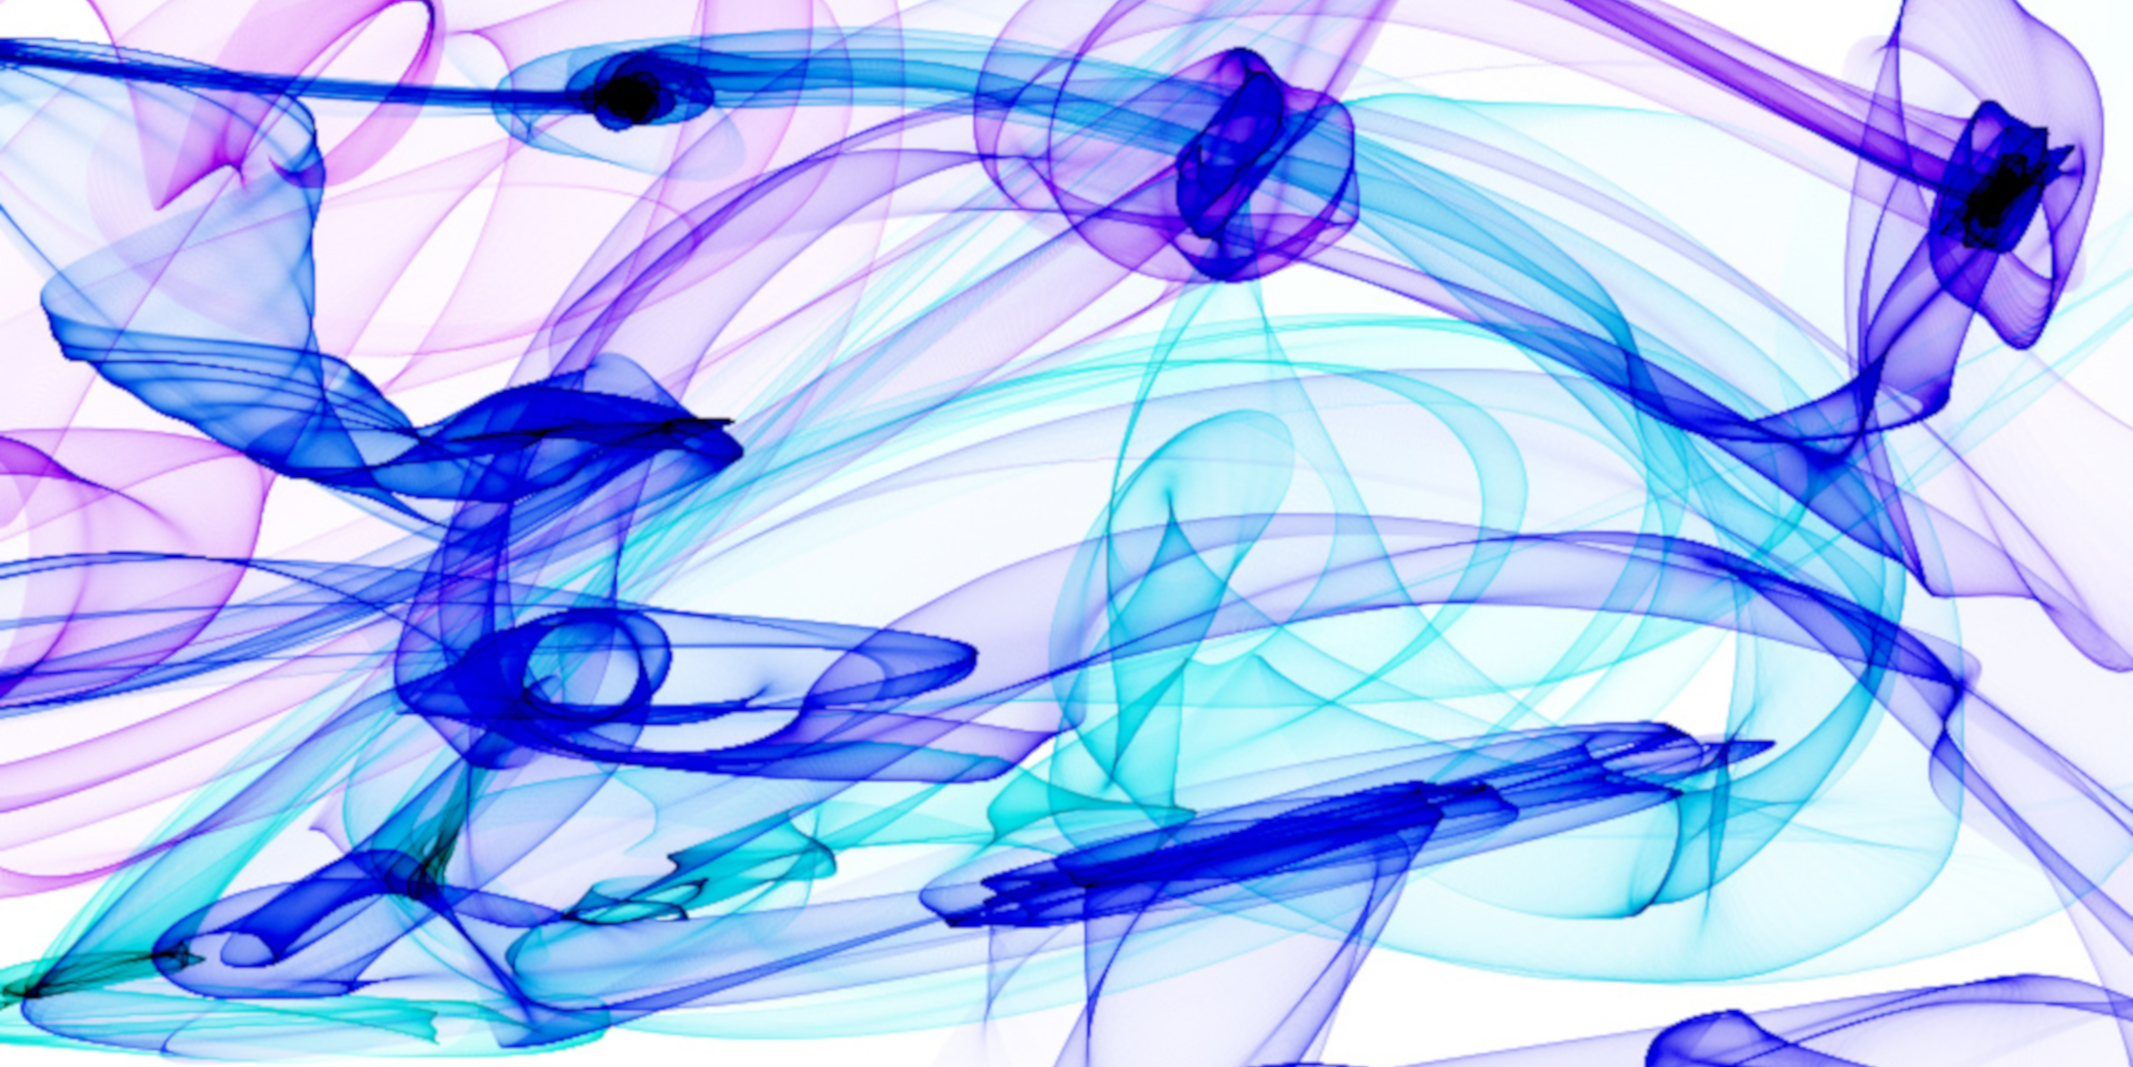
\includegraphics[scale=0.1]{Pictures/FlameArtwork2}
\caption{Come includere una figura, salvata nella cartella immagini.}\label{fig:figura}
\end{figure}




\chapter{Il barometro}
\section{Generalit\`a}
In questa sezione proviamo a modificare l'INTERLINEA.\\

\begin{interlinea}{0.87}
Il barometro, come dice il nome, serve per misurare la pesantezza; pi\`u precisamente la pesantezza dell'aria riferita all'unit\`a di superficie.
\end{interlinea}

\begin{interlinea}{2}
Studiando il fenomeno fisico si pu\`o concludere che in un dato punto grava il peso della colonna d'aria che lo sovrasta, e che tale colonna \`e tanto pi\`u grave quanto maggiore \`e la superficie della sua base; il rapporto fra il peso e la base della colonna si chiama pressione e si misura in once toscane al cubito quadrato, \cite{tor1}; nel Ducato di Savoia la misura in once al piede quadrato \`e quasi uguale, perch\'e col\`a usano un piede molto grande, che \`e simile al nostro cubito.
\end{interlinea}

\subsection{Forma del barometro}
Il barometro consta di un tubo di vetro chiuso ad una estremit\`a e ripieno di mercurio, capovolto su di un vaso anch'esso ripieno di mercurio; mediante un'asta graduata si pu\`o misurare la distanza fra il menisco del mercurio dentro il tubo e la superficie del mercurio dentro il vaso; tale distanza \`e normalmente di 10 pollici toscani, \cite{tor1,tor2}, ma la misura pu\`o variare se si usano dei pollici diversi; \`e noto infatti che gl'huomini sogliono avere mani di diverse grandezze, talch\'e anche li pollici non sono egualmente lunghi.

\section{Del mercurio}
Il mercurio \`e un a sostanza che si presenta come un liquido, ma ha il colore del metallo. Esso \`e pesantissimo, tanto che un bicchiere, che se fosse pieno d'acqua, sarebbe assai leggiero, quando invece fosse ripieno di mercurio, sarebbe tanto pesante che con entrambe le mani esso necessiterebbe di essere levato in suso.


\setcounter{footnote}{25}

Il Monte Amiata, che \`e locato nel territorio del Ducato%
\footnote{Naturalmente stiamo parlando del Granducato di Toscana.%
\ifclassica\NoteWhiteLine\fi
} del nostro Eccellentissimo et Illustrissimo Signore Granduca di Toscana\footnote{Cosimo IV de' Medici.}, \`e uno dei luoghi della terra dove pu\`o rinvenirsi in gran copia un sale rosso, che nomasi \emph{cinabro}, dal quale con artifizi alchemici, si estrae il mercurio nella forma e nella consistenza che occorre per la costruzione del barometro terrestre%
\ifclassica
\nota{Nota senza numero\dots

\dots e che va a capo.
}\fi.

La densit\`a del mercurio \`e molto alta e varia con la temperatura come pu\`o desumersi dalla tabella \ref{t:1}.

\begin{table}[htp]              
\centering                      
\begin{tabular}%                
{r c l p{5cm}}                  % parametri di incolonnamento: r (a destra), c (al centro), l (a sinistra),
								% p (per definire la larghezza della colonna)
\hline\hline
Colonna 1 & Colonna 2 & Colonna 3 & Colonna 4 \\  
\hline
\hspace*{1.3em}
  & 10  & 100 & 13,8  \\
2 & 20  &     & 13,6  \\
  & 30  & 300 & 13,5  \\
4 & 40  &     & 13,3  \\
\hline \hline
\end{tabular}
\caption[Descrizione breve: compare nell'elenco tabelle]{Descrizione completa: didascalia della tabella.} \label{t:1}  
%[Short description for the content list.]{Complete descreption: caption of the table.}
\end{table}



\begin{table}[htp]              
\centering                      
\begin{tabular}{d d}                        
\hline\hline                    
\multicolumn{1}{c}{Temperatura} & \multicolumn{1}{c}{Densit\`a}  \\  
\multicolumn{1}{c}{\unit{\gradi C}} & \multicolumn{1}{c}{$\unit{t/m^3}$}  \\
\hline%                        
\hspace*{1.3em}
0 & 13.8 \\   
10 & 13.6 \\   
50 & 13.5 \\   
100 & 13.3 \\   
\hline \hline
\end{tabular}
\caption[Densit\`a del mercurio]{Densit\`a del mercurio. Si pu\`o fare molto meglio usando il pacchetto \textsf{booktabs}.} \label{t:2}  % didascalia con label
\end{table}


\begin{osservazione}\normalfont
Questa propriet\`a si manifesta quando esso \`e estremamente freddo, come quando lo si immerge nella salamoia di sale e ghiaccio che usano li maestri siciliani per confetionare li sorbetti, dei quali sono insuperabili artisti.
\end{osservazione}
%
\begin{observation}\normalfont
This is the English version of \emph{Osservazione}.
\end{observation}

Per nostra fortuna, questo grande freddo, che necessita per la confetione de li sorbetti, molto raramente, se non mai, viene a formarsi nelle terre del Granduca Eccellentissimo, sicch\'e non vi ha tema che il barometro di mercurio possa essere ruinato dal grande gelo e non indichi la pressione giusta, come invece deve sempre fare uno strumento di misura, quale \`e quello che \`e descritto cost\`i \cite{duane1964}.


\chapter{Kubernetes}
(CITA https://kubernetes.io/docs/concepts/overview/  METTERLA COME CITAZIONE TRA VIRGOLETTE?)
Kubernetes is a portable, extensible, open source platform for managing containerized workloads and services, that facilitates both declarative configuration and automation


Kubernetes emerged as a platform designed to automate the management of containerized applications, ensuring periodic checks to maintain alignment between the actual operational state and the defined ideal state through a declarative language. A decade since its release as an open-source project, Kubernetes stands as one of the most extensively utilized platforms worldwide. This project focuses on k3s, a lightweight variant of Kubernetes tailored for operation in resource-constrained environments.

\section{Basic concepts}
The foundational principles underlying the architecture of Kubernetes are articulated as follows:
\begin{enumerate}
\item Implementation-agnostic APIs: Each Kubernetes object can be implemented differently depending on the version being used, yet the interface used to manage these objects remains consistent across all versions.
\item Completely declarative specification: Kubernetes facilitates the use of a declarative language instead of the traditional imperative approach, simplifying application management by specifying the desired state directly rather than detailing how to achieve that state from various starting points.
\item Control loop-oriented approach: Kubernetes employs components known as controllers that cyclically monitor whether the current state aligns with the desired state. If discrepancies are identified, these controllers initiate actions to minimize the gap between the states.
\end{enumerate}
These principles are the cornerstone of Kubernetes, facilitating efficient management and orchestration of containerized applications in a variety of computing environments.

Every object within Kubernetes is meticulously crafted to adhere to foundational principles, starting with its smallest operational unit: the pod. A pod may consist of one or more containers and its configuration is defined in its respective YAML file. This file may reference other configuration files using key-value pairs, such as Secrets or ConfigMaps, useful in case these configurations are repeated multiple times. 
Pods are typically instantiated through the implementation of various Kubernetes controllers.

The Deployment controller, commonly used for stateless applications, describes the desired application state while managing scalability through the ReplicaSet. For stateful applications, the StatefulSet controller is normally utilized, managing the pod-to-volume binding and ensuring properties such as unique network IDs that the stateful application required to function properly.
While controllers oversee the lifecycle of pods, pod discovery is entrusted to Services. These Kubernetes objects target all pods matching their selector criteria, facilitating exposure both within and outside the cluster. ClusterIP services expose pods solely within the cluster, whereas NodePort or LoadBalancer services extend pod accessibility externally.
Pods are instantiated on physical or virtual machines known as nodes, which serve either as master or worker nodes based on their role. A master node not only executes various Kubernetes components, as previously discussed, but also hosts the cluster's control plane such as the scheduler, controller manager, and API server. Conversely, a worker node is dedicated solely to executing the workloads of Kubernetes objects.
The cluster, comprising these nodes, can be structured as a single-master or multi-master configuration. In a multi-master setup, control plane components are replicated across all master nodes, with decisions made via a consensus mechanism based on a quorum(CITA QUALCOSA?). This setup necessitates an odd number of master nodes to prevent split-brain(CITA WIKIPEDIA O RICERCA?) scenarios and reduce decision-making delays. These structural and operational principles form the backbone of Kubernetes architecture, facilitating scalable and efficient container orchestration in diverse computing environments.

\section{K3s}
K3s is a lightweight variant of Kubernetes tailored for operation in resource-constrained environments, for example its binary file is less than 100Mb. This is achieved deleting some legacy libraries, using sqlite3 instead of the standard etcd as database manager (this is the default choice, other as the same etcd are available and can be configured). The installation is done by using a simple script, that will handle most of the complicancy of kubernetes environment as setting TLS certificate automatically.




\chapter{Liqo}
Due to the rapid adoption of containers as the development environment for applications, there is now a well-established trend towards using orchestration platforms to automate the lifecycle management of containerized applications. 

Among the various implementations of these platforms, Kubernetes has gained predominant traction, to the extent that multinational corporations with dedicated cloud departments (such as Google, Amazon, Microsoft, Alibaba...) have developed proprietary solutions based on it. 

Recently, a trend similar to the one observed with container adoption has emerged, in which there is a growing need for a system that can automate relationships between various clusters managed by these platforms, whether in the cloud or on-premise. 

In this chapter will be summarized the Liqo project, designed to address this necessity, described by its creators \cite{l0-1} as "an open-source project that enables dynamic and seamless Kubernetes multi-cluster topologies, supporting heterogeneous on-premise, cloud, and edge infrastructures."

\section{Basic concepts}
The Liqo technology facilitates the creation of a unified virtual network across diverse clusters, enabling the execution of application pods on remote clusters as if they were local. This system is founded on four primary characteristics: network fabric, peering, offloading, storage fabric.

\subsection{Network fabric}
The network fabric is the subsystem of Liqo that seamlessly extends the Kubernetes networking model across multiple independent clusters, enabling pods on different clusters to communicate smoothly even when address NAT is applied.

The control plane of this subsystem resides in the network manager, instantiated as a pod responsible for managing network parameters. It handles tasks both during cluster peering and inter-cluster communications, as example featuring an interface used by the reflection logic for IP address translation.

Interconnecting two clusters involves deploying a secure VPN tunnel using WireGuard, typically established at the end of the peering process based on negotiated parameters. This functionality is implemented by the Liqo gateway component, operating within the cluster as a privileged pod. It also manages routing tables and configures necessary NAT rules to resolve address conflicts. 

Although initialized within the cluster's network, this pod utilizes a separate network namespace and policy routing to avoid conflicts with Kubernetes' existing Container Network Interface (CNI) plugins.

Traffic from local nodes/pods directed to a remote cluster is routed through an overlay network, based on VXLAN, managed by a DaemonSet component. This component is responsible for routing entries and ensures proper handling of traffic across the VPN tunnels.

\subsection{Peering}
Standard peering is the process that establishes a unidirectional link between two different Kubernetes clusters, enabling the sharing of resources and services. Through this connection, the consumer cluster can initiate processes using resources provided by the provider cluster, but not vice versa. 

In this context, the consumer cluster initiates an outgoing peering towards the provider, which reciprocates with an incoming peering from the consumer. This linkage is not exclusive, supporting possible bidirectionality and the scenario where a cluster can act as a consumer for some peerings and as a provider for others.

The peering process unfolds through the following steps:
\begin{enumerate}
\item Authentication: Each cluster uses a pre-shared token to verify its identity, which has some permissions for Liqo-related resources and negotiations.
\item Parameter Negotiation: The two clusters exchange sets of parameters necessary for finalizing the peering, including network information such as their respective CIDRs or as the amount of resources shared by the provider. 

Some of these parameters can be modified directly or using dedicated plugins, for example is possible adjusting the available resources that the provider cluster shows to the consumer cluster.
\item Creation of the Virtual Node: Within the consumer cluster, a virtual node is created to represent the resources shared by the provider cluster. Processes instantiated using the provider cluster's resources appear to be located within this virtual node, maintaining transparency in the offloading process and adhering to standard Kubernetes practices without requiring API modifications.
\item Configuration of the Network Fabric: The two clusters configure their respective network fabrics and establish a secure VPN tunnel using the previously negotiated parameters (address remapping, endpoints, etc.).
\end{enumerate}
Each connection can be differentiated based on how Liqo's control plane traffic is managed: whether it passes through the VPN tunnel alongside pod traffic (in-band control plane peering) or uses traditional communication channels (out-of-band control plane peering). 

In the former case, it is required to expose only the Liqo VPN endpoint to the pod of the remote cluster. However, this setup requires control over both clusters to negotiate network parameters through Liqo CTL tool \cite{l1-1}, resulting in a static peering configuration that requires manual intervention for updates. 

In the latter case, while to the remote pods must be expose not only the Liqo VPN endpoint but also the Kubernetes API and Liqo authentication service endpoints (as shown in the Figure \ref{fig:out-band}), it offers the flexibility to connect clusters across different domains using a pre-shared token and enables dynamic peering, so that an automatic renegotiation of parameters occurs in response to configuration changes. 

\begin{figure}[ht]\centering
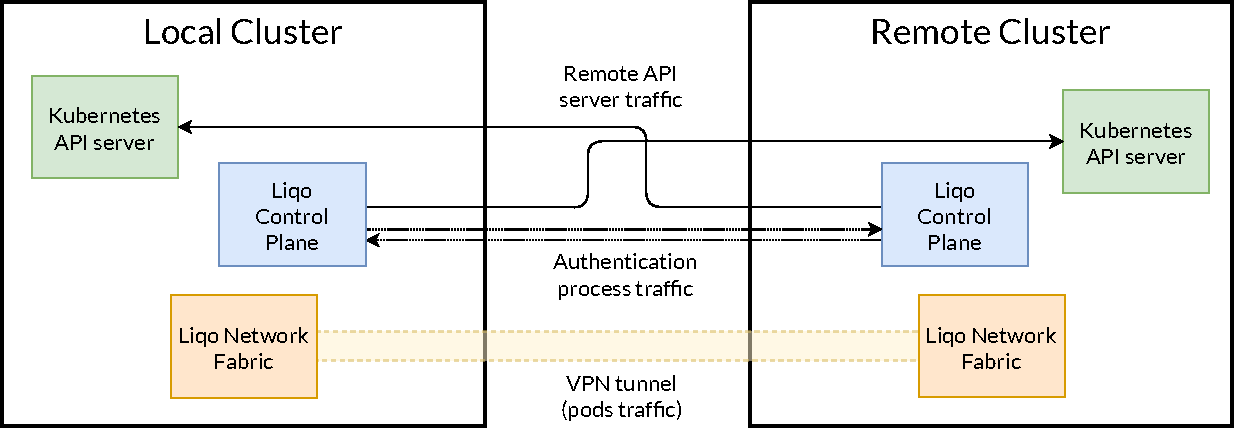
\includegraphics[scale=.5] {Pictures/out-of-band}
\caption{Out-of-band control plane peering}\label{fig:out-band}
\end{figure}

\subsection{Offloading}
Offloading is the method enabling transparent extension of the local cluster into a remote cluster, allowing Kubernetes scheduler to seamlessly schedule workloads in the remote cluster when it's deemed optimal. The virtual node is managed by an extended version of the Virtual Kubelet project, which replaces the traditional kubelet if the node isn't physical. 

In the context of Liqo, it interacts with the Kubernetes API servers of both clusters to manage artifact propagation (pods, services, config maps) and reconcile state in case of changes on the negotiated configurations. It also performs configurable periodic health checks to assess reachability of the remote API server, marking the node as unready in case of repeated failures and triggering standard Kubernetes evacuation strategies. 

An instance of the virtual kubelet is created for each remote cluster to ensure isolation and segregation of authentication tokens.

The offloading process comprises three stages:
\begin{enumerate}
\item Namespace Extension: The local cluster's namespace is extended into the remote cluster by creating a gemini counterpart namespace, which will host both offloaded pods and resources required for pod reflection.
\item Resource Reflection: Selected arctifacts from the control plane are reflected in remote clusters to ensure the operational functionality of the pods. Supported resources for reflection include service exposure (Ingress, Services, EndpointSlices), persistent storage (PersistentVolumeClaims, PersistentVolumes), and configuration data (ConfigMaps, Secrets).
\item Pod Offloading: After the scheduler schedules a pod on the virtual node, the corresponding virtual kubelet creates a mirrored pod object in the remote cluster. This object is managed by the custom resource ShadowPod~\cite{l1-2}, serving as a representation of the pod to maintain service functionality even if connectivity with the remote cluster is lost.
\end{enumerate}
Both stateless and stateful pods are supported, with the latter utilizing either the storage fabric or relying on an external volume provider.

\subsection{Storage fabric}
The storage fabric is the Liqo subsystem responsible for managing the creation of remote volumes for stateful applications. Its operation revolves around delaying the binding of a volume to a pod until it has been scheduled to a node, ensuring volumes are always created where their associated pod is scheduled. 

Subsequent scheduling adheres to a data gravity principle, transparently rescheduling the pod to the node where the physical volume resides. These behaviors are implemented through Liqo's virtual storage class, utilizing reflection mechanisms when pods are scheduled on virtual nodes to create the mirrored PVCs in remote clusters. Alternatively, it relies on the real storage class when pods are scheduled on local physical nodes.

\section{Distributed DB interaction}
At present, most of the distributed database systems doesn't support general multi-cluster architecture, primarily due to their reliance on internal headless services for direct pod-to-pod communication. These services return the IP address of the corresponding pod directly when queried, using their DNS entry, unlike regular services that route requests via kube-proxy. 

Liqo employs an address remapping mechanism to facilitate seamless communication between clusters; however, this approach results in incorrect IP resolutions for pods scheduled on remote clusters when queried by headless services.

To enable the use of these architectures, Liqo developers currently recommend\cite{l2-1} leveraging the peering process, which exposes the address ranges of the two clusters in two different ways:
\begin{enumerate}
\item Connecting a cluster to all others via peering while forcing a pod of the distributed system onto it: This approach ensures that the service in that cluster is aware of all real address ranges, allowing replication through the forced pod, which becomes a critical point.
\item Creating a full mesh of peering between various clusters: This ensures that each headless service knows the addresses of all others, and this is the solution adopted in this research.
\end{enumerate}
Some distributed database architectures, such as those implemented by the Percona XtraDB Cluster Operator, may introduce additional complexity. After receiving the translated IP of a remote pod, they may encounter difficulties establishing a connection, primarily because their cluster logic operates with standard Kubernetes component independently of Liqo. This requires the implementation of distinct CIDRs across clusters, ensuring that traffic is routed through Liqo components to establish connections correctly.

\chapter{General architecture domain mesh}
In questo capitolo si descriverà il percorso che ha portato alla creazione dell'architettura domain mesh, modello in grado di applicare i paradigmi logici del edge/fog computing ad una architettura multi-cluster garantendo al tempo stesso la possibilità di deployare sistemi high-availability. Inizialmente verranno discusse le scelte strutturali, basate sia sull'ambiente multi-cluster sia sui requisiti delle tecnologie adottate (Percona, Liqo..). Si passerà successivamente alla descrizione di possibili casi d'uso, mostrando la flessibilità delle architetture gerarchiche logiche che si possono implementare. Infine si valuteranno le caratteristiche e le varie limitazioni che questo modello comporta. 

\section{Physical/net architecture}
Il modello Domain Mesh (cambiare domain mesh a stella estesa?) si può rappresentare come una topologia stella estesa(CITA figura con spiegazioni come nodi=cluster)
La rete di controllo e monitoraggio dell'energia elettrica si pùò schematizzare con un grafico appartenente alla topologia ad albero (CITA come aggiungere che i nodi intermedi possono fare operazioni ma hanno limitato spazio perciò non full controllo-> peer-to-peer da scartare?), e tra queste topologie il modello a stella è l'unico che possa essere implementato fisicamente utilizzando la versione standard di Liqo. Difatti essa non permette l'offloading di un namespace già offlodato, per evitare che si possano creare situazioni critiche come offloading circolari. Questo comporta che tutte le topologie gerarchiche a più livelli non possano essere implementate fisicamente senza apportare cambiamenti personalizzati al codice della tecnologia. Inoltre i sistemi di database distribuiti HA tendono ad aver bisogno di essere in un unico namespace, e le soluzioni multinamespace tramite operatori non supportano tecnologie multicluster in quanto non possono conoscere i namespace di altri cluster.
La versione estesa del modello stella, la quale permette collegamenti diretti tra foglie, è necessaria per il corretto funzionamento trasparente multicluster per i sistemi di database distribuito che si basano su servizi headless. Ogni cluster che utilizzi il sistema di database necessiterà infatti, oltre di un essere in un unico namespace, di agire nello stesso namespace e di un collegamento diretto con tutti gli altri cluster, creando per il dominio del database una topologia mesh parziale (parziale in quanto i collegamenti non devono necessariamente essere bidirezionali).

\section{Logic hierarchy with labels and affinity}
Una semplice topologia a stella estesa non ha la flessibilità necessaria per gestire i differenti casi reali in cui si articola una rete di monitoraggio, ordunque si rende necessaria l'introduzione di una strategia per costruire una topologia logica complessa sul modello fisico esistente. Questa strategia si basa sull'utilizzo dei meccanismi di label e affinità nativi di Kubernetes: Ogni cluster sarà identificato da un gruppo di label, le quali specificheranno la posizione di esso nella topologia logica desiderata e che potranno essere utilizzate dallo scheduler per distribuire secondo la logica desiderata il carico di lavoro. Si utilizza il meccanismo di node affinity sia per distinguere i vari cluster, sia per distinguere i vari nodi in un cluster, mentre la pod affinity si utilizza nel caso si voglia inserire qualche condizione di esistenza tra pod nello stesso nodo. In caso di sistemi che utilizzino servizi headless, ogni cluster all'interno di un gruppo dovrà avere un peering con tutti gli altri per permetterne il funzionamento.
Le prossime sottosezioni tratteranno alcune topologie logiche di base, dalle quali si può partire per costruire la propria desiderata. 

\subsection{Groups indipendent/domain}
In questa topologia si suddividono i clusters foglia in gruppi tramite l'assegnazione della label identificativa del gruppo. In questo modo si ottengono diverse aree logiche a cui si possono assegnare diversi carichi di lavoro. Questi gruppi, se non esiste nessun contraddizione logica tra le label identificative, non sono esclusivi, perciò un cluster potrebbe far parte di più gruppi contemporaneamente.

\subsection{Groups dependent/levels}
Questa tipologia mostra il modo più semplice per creare una gerarchia tra i gruppi. Ogni gruppo, oltre alla label identificativa del proprio dominio, avrà una label inerente al posizionamento dello stesso nella gerarchia logica, supportando perciò nuovi comportamenti come il permettere non solo la scelta su quali gruppi schedulare il carico di lavoro ma anche su quali cluster nel gruppo

\section{Extended Star Analysis}
Come illustrato precedentemente, la topologia a stella estesa permette di utilizzare sistemi non pensati per l'uso multicluster come i database distribuiti HA, implicando però al contempo una crescita quadratica (CITA metti formula full mesh numero link) del numero di peering necessari tra i cluster nel dominio del database. Il crescere del numero dei peering affligge solamente il tempo necessario per setuppare l'intera archittetura nel momento della creazione, in quanto il consumo di risorse aggiuntive risulta trascurabile (CITA PAPER?). 
Lo sfruttamento del meccanismo delle label invece permette un'enorme flessibilità nella scelta dell'architettura logica da sovrapporre a quella fisica, con il solo svantaggio di aumentare, esponenzialmente all'aumentare della complessità della topologia logica o linearmente all'aumentare del numero di cluster, il tempo di setup dell'architettura.
Questo comporta che la topologia a stella estesa è ottimale per sistemi relativamente stabili, permettendo al contempo la possibilità di piccoli cambiamenti logici on the fly oppure di grandi cambiamenti topologici al costo di un certo tempo di setup


\chapter{Possible implementations}
This chapter will discuss the potential implementations of the partial mesh star topology within the context of a computer network dedicated to energy monitoring. The network primarily consists of the Area Control Center, primary stations, and secondary stations, each managed by its own Kubernetes cluster.

\section{Logical domains}
This implementation is depicted in Figure~\ref{fig:domains}, where the Area Control Center occupies the central position in the star topology, establishing unidirectional peering with offloading to every other entity in the topology, whether it is a primary station or a secondary station.

\begin{figure}[ht]\centering
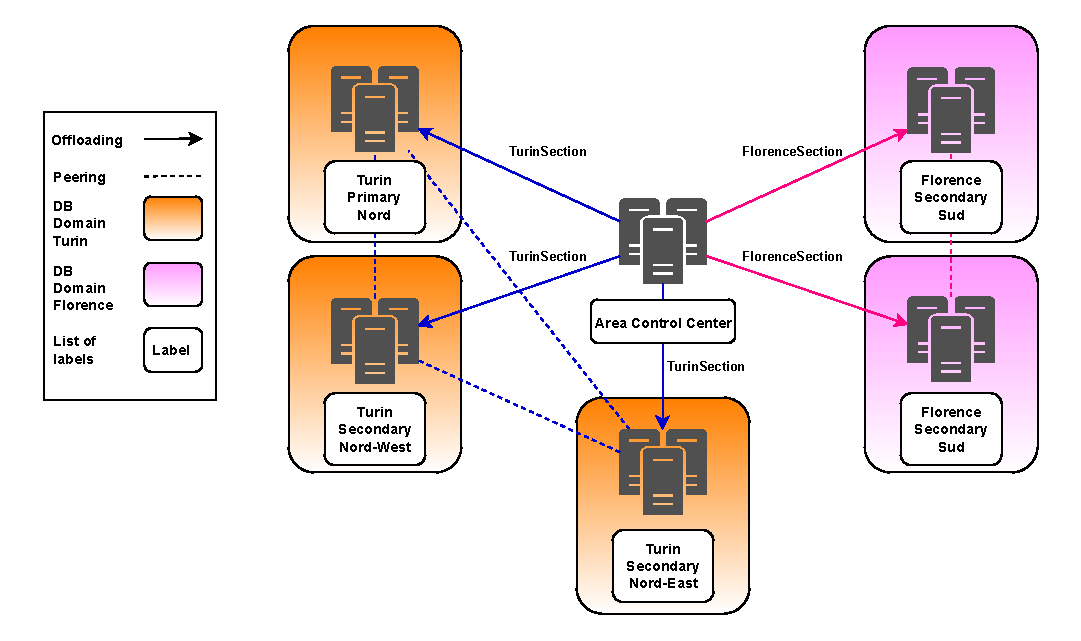
\includegraphics[scale=0.7]{Pictures/Domain-v3}
\caption{Logical domains scheme.}\label{fig:domains}
\end{figure}

This allows the Area Control Center to manage all application deployments without the need to delegate them to other nodes.
The remaining clusters are divided into groups, typically consisting of a primary station and its associated secondary stations. These groups represent a logical domain of applications with their own high-availability distributed database system and, therefore, do not have interconnections among them. Within a group, the clusters form a full mesh of unidirectional peerings for the database system's operation, and they share the same offloaded namespace from the Area Control Center. 


\subsection{Logical domains analysis}

This architecture allows for the highest degree of resilience, as considering every possible failure in the control and power distribution network infrastructure, represented in Figure~\ref{fig:failures}, the only fault that is not automatically recoverable is the disconnection of the Area Control Center.

\begin{figure}[ht]\centering
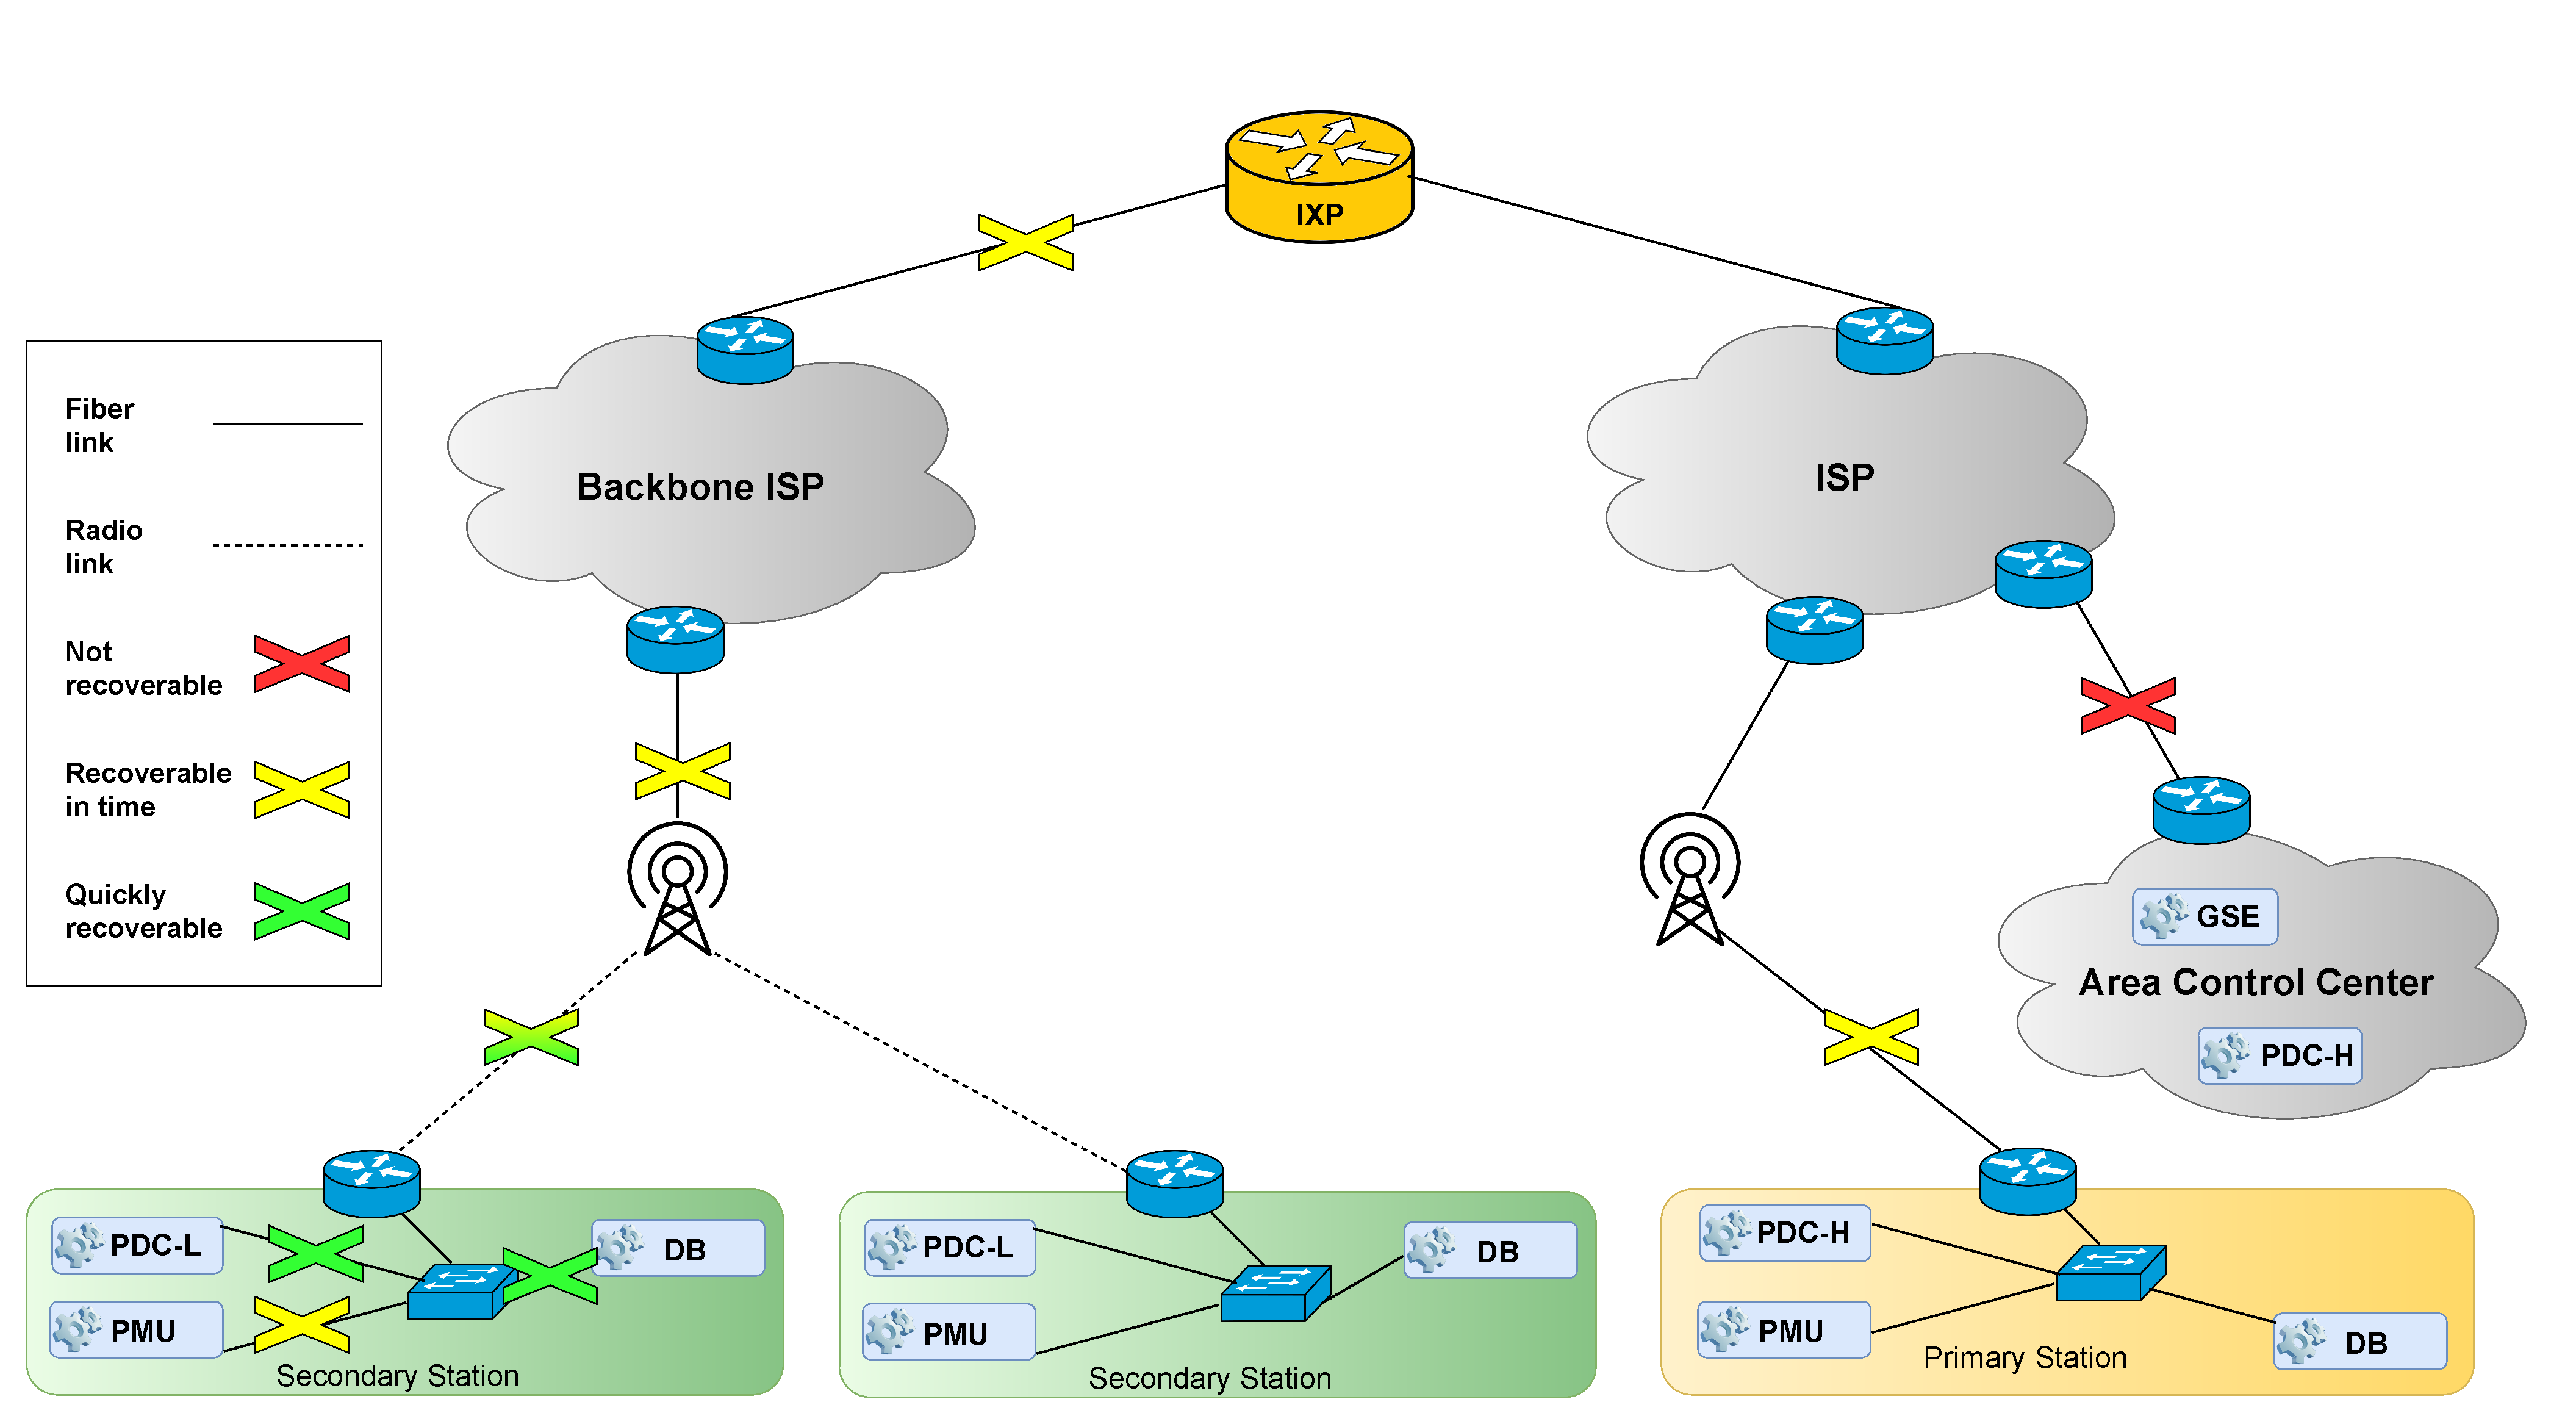
\includegraphics[scale=0.20]{Pictures/failures}
\caption{Possible failures in logical domains implementation.}\label{fig:failures}
\end{figure}

The cluster representing the Area Control Center is a critical point as it hosts the central logic of the network, but the effects of a failure or disconnection of this node are negligible when compared to environmental constraints:

\begin{enumerate}
\item In the event of a physical failure of the central node, deployments would be lost, making the reconciliation process with the entire network impossible. However, this is negligible because without the central node's logic, the network would not be observable by default.
\item In the event of a complete disconnection from the network, active workloads would continue to function, but the reconciliation process for stateful applications (as the database system) will not occur since, by the point of view of the deployments, there would not be enough surviving replicas to maintain the system. Yet, this is also negligible as it falls under the same scenario as before.
\end{enumerate}

In contrast, all other failures are recoverable from the perspective of the Area Control Center. Failures within a cluster are generally recoverable in a short time as the applications are automatically and quickly ricreated into a healthy node (which can belong to either the local cluster or a remote cluster) in case of disconnection or internal pod failure. 

Disconnections of nodes, entire clusters, or parts of the network containing data production sources (PMUs) are automatically recoverable only with the restoration of the connection itself, as the PMU is physical hardware tied to its node and cannot be moved to others.

The aforementioned concerns the perspective of the Area Control Center, but as described in the previous chapter, the disconnected part of the network continues to function perfectly, and thanks to Liqo technology, additional applications can be instantiated to support the temporary independence of the network.

The continuation of operations can be observed in Figure~\ref{fig:stream}, which illustrates the data stream about frequency values seen by an instance of PDC lower and its directly superior PDC higher, shortly before and shortly after the disconnection of the cluster hosting the PDC lower and its data sources, which occurred at 44,633 s. PDC lower continues to receive data from the sources, operating in an isolated environment, while PDC higher stops receiving the data stream from the isolated source. 

\begin{figure}[ht]\centering
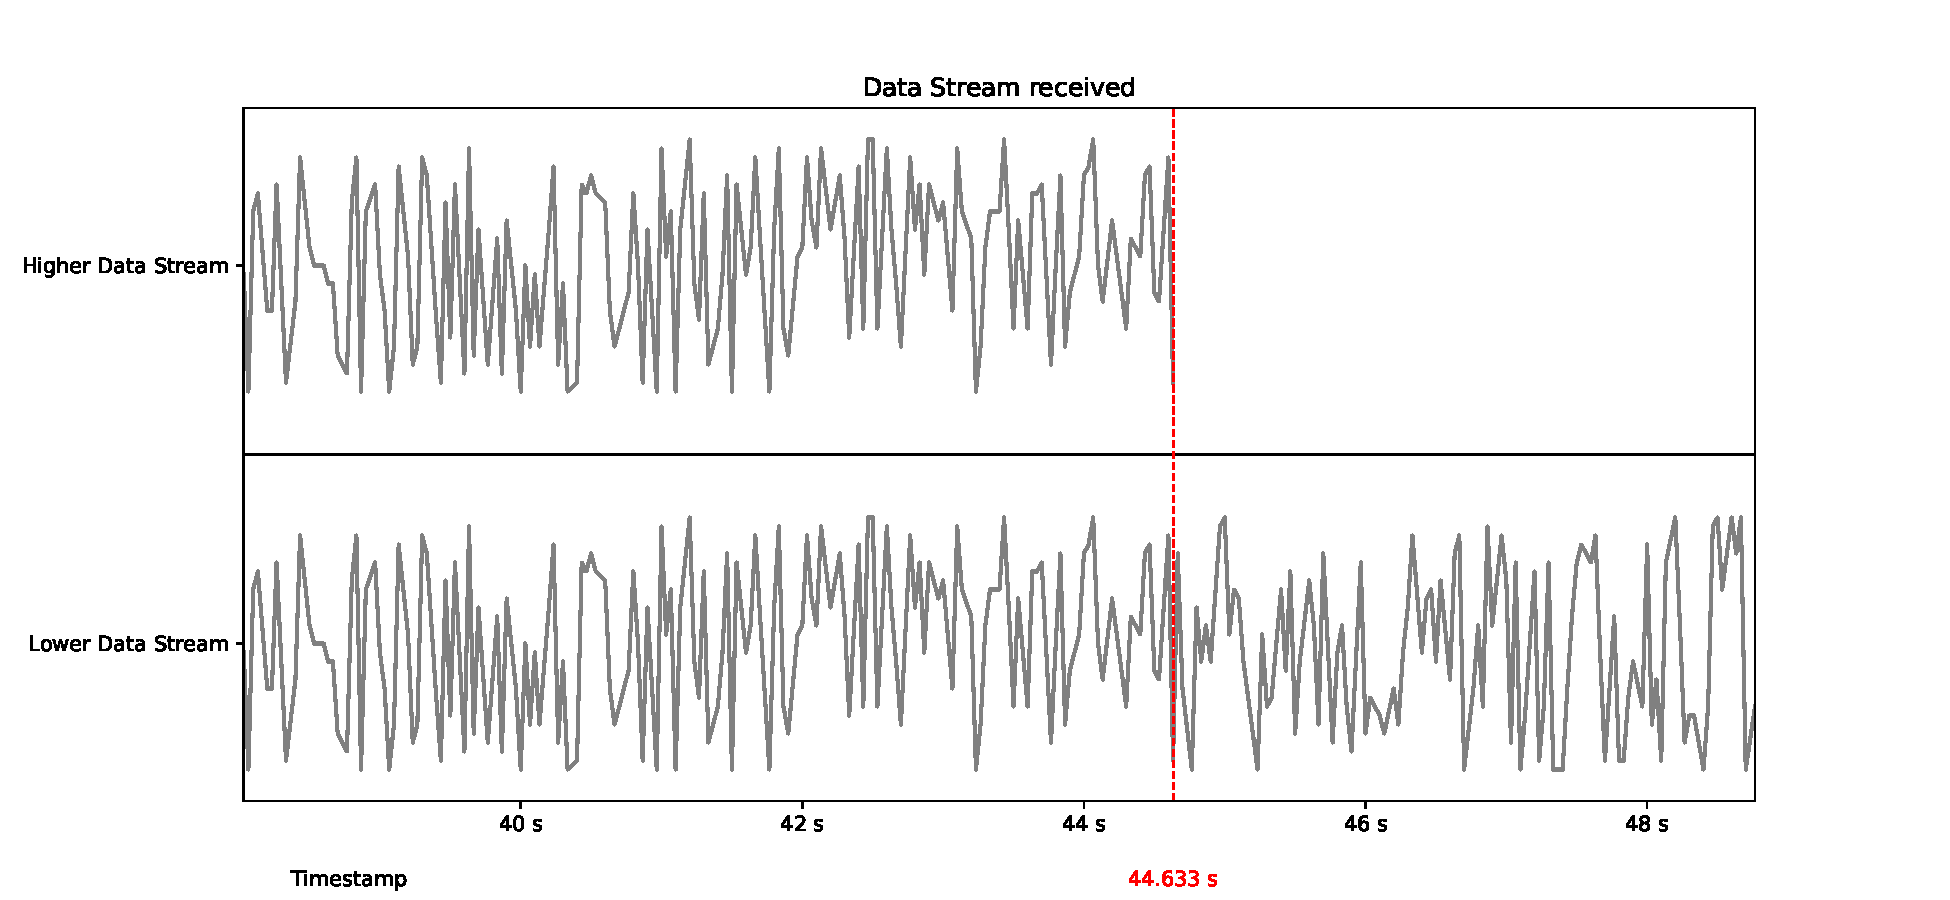
\includegraphics[scale=0.5]{Pictures/data-stream}
\caption{Data Stream comparison in case of failure.}\label{fig:stream}
\end{figure}

Comparing the risks arising from the failure of one component with those that an extended local solution encompassed, as shown in Table ~\ref{t:6}, it can be noted that many have decreased, as there is no longer the possibility of the network remaining unobservable. The risks related to PMU failures have remained the same, as it cannot be rescheduled to another node.

\begin{table}[ht]              
\centering 
\begin{tabularx}{\textwidth}{|l|c|X|}
\hline
\textbf{Component Failure} & \textbf{Severity} & \textbf{Cause}\\ 
\hline
\raisebox{-0.75cm}{Single PMU} & \raisebox{-0.75cm}{Low-> Low} & Generally the number of other PMUs guarantees the observability threshold. \\
\hline
\raisebox{-0.75cm}{Multiple PMUs} & \raisebox{-0.75cm}{Low-High-> Low-High} & It depends on whether the number of other PMUs guarantees the observability threshold.\\
\hline
\raisebox{-0.75cm}{Single PDC-l} & \raisebox{-0.75cm}{Moderate-High-> Low-Moderate} & The observability of the network is impaired until the PDC is rescheduled onto another node.\\
\hline
\raisebox{-0.75cm}{Multiple PDCs-l} & \raisebox{-0.75cm}{Moderate-High-> Low-Moderate} & The observability of the network is impaired until the PDCs are rescheduled onto another nodes. \\
\hline
\raisebox{-0.75cm}{Single PDC-h} & \raisebox{-0.75cm}{High-> Moderate}& The observability of the network is impaired until the PDC is rescheduled onto another node. \\
\hline
\end{tabularx}
\caption[Component failures on Logical Domains topology overview.]{Component failures on Logical Domains topology overview.} \label{t:6}  
\end{table}

The limitations of this architecture pertain to scalability, as each cluster requires its own distinct CIDR for the transparent operation of high-availability distributed database systems. Additionally, each peering creates a virtual representative node in the central cluster, limiting the number of possible clusters to 5000, according to the official Kubernetes documentation.

\section{Multi-level logical domains}
The implementation described in this section leverages a star topology twice, once with a partial mesh version and once with a full version, as shown in Figure~\ref{fig:level-imp}. This follows the division of stations into primary and secondary, although it could be adapted to n subdivisions.

\begin{figure}[ht]\centering
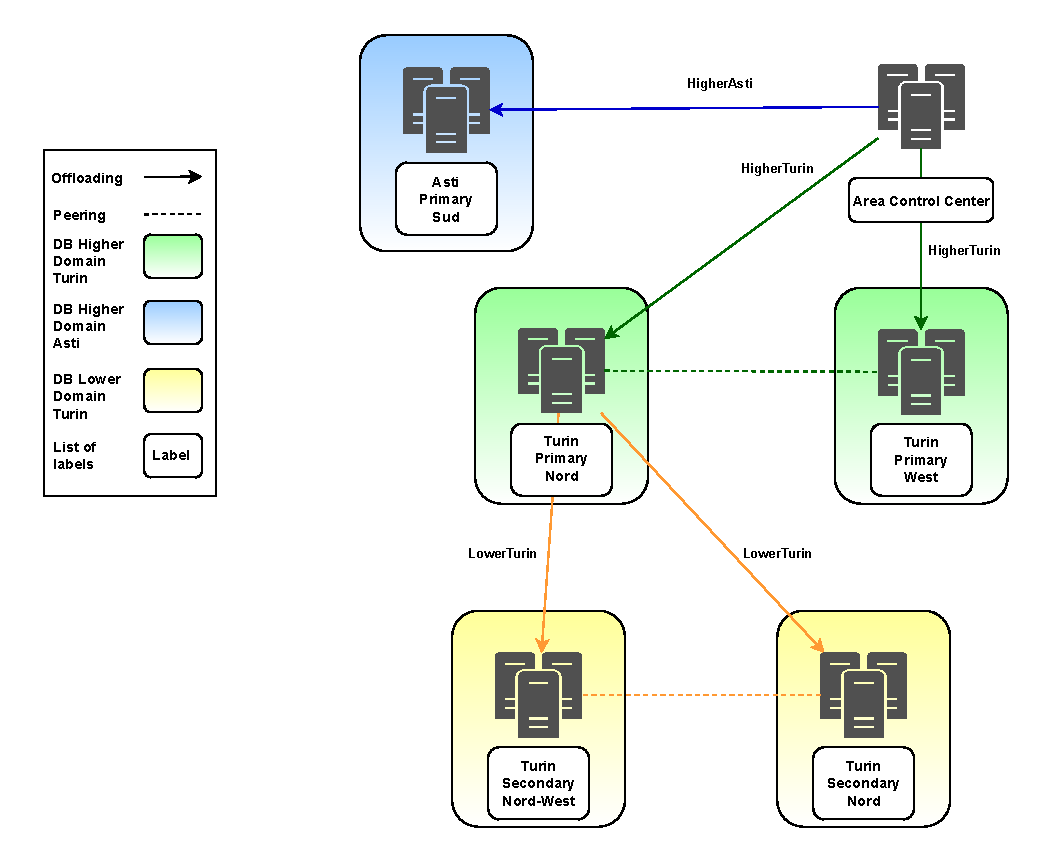
\includegraphics[scale=0.7]{Pictures/2level}
\caption{2 Level logical domains.}\label{fig:level-imp}
\end{figure}

The first topology used is a partial mesh star topology used to connect the Area Control Center (central cluster) with all primary stations (leaf clusters). The central cluster handles the deployment of high-level applications along with their respective distributed database systems, offloading the corresponding namespace through peering to the respective group of primary stations.

The groups of primary stations are composed of a main primary station, where workload is preferably directed (using labels), while the others in the group primarily serve as backups in case of failure of the main station. This means that primary stations can be in multiple groups, one where they are primary and others where they function as backups, leveraging the topology seen in Chapter~\ref{chap:partial-mesh-star} section~\ref{sec:indipendent-groups}.

The main primary station of each group also serves as the central cluster in the second star topology, connecting not only to the backup primary stations but also to all secondary stations under its jurisdiction. In our implementation, this will be a full mesh star topology, but a partial mesh could also be used if the secondary stations do not share the same distributed database system.

In this second topology, the main primary station handles the deployment of low-level applications along with their respective high-availability distributed databases, consequently offloading the namespace to its secondary stations. The data stream for monitoring, which passes through two different namespaces (from the low-level to the high-level), relies on external exposure services such as load balancers and ingress, enabling access to the high-level application whether it resides in the primary station or, due to a failure, in one of the backup primary stations.


\subsection{Multi-level Logical domains analysis}

This architecture enhances scalability limits compared to the previous implementation by reducing the number of peerings managed by the Area Control Center,  as shown in Figure~\ref{fig:failures2}, and by requiring distinct CIDRs only within the secondary topologies associated with a primary station, allowing for reuse across different types.

\begin{figure}[ht]\centering
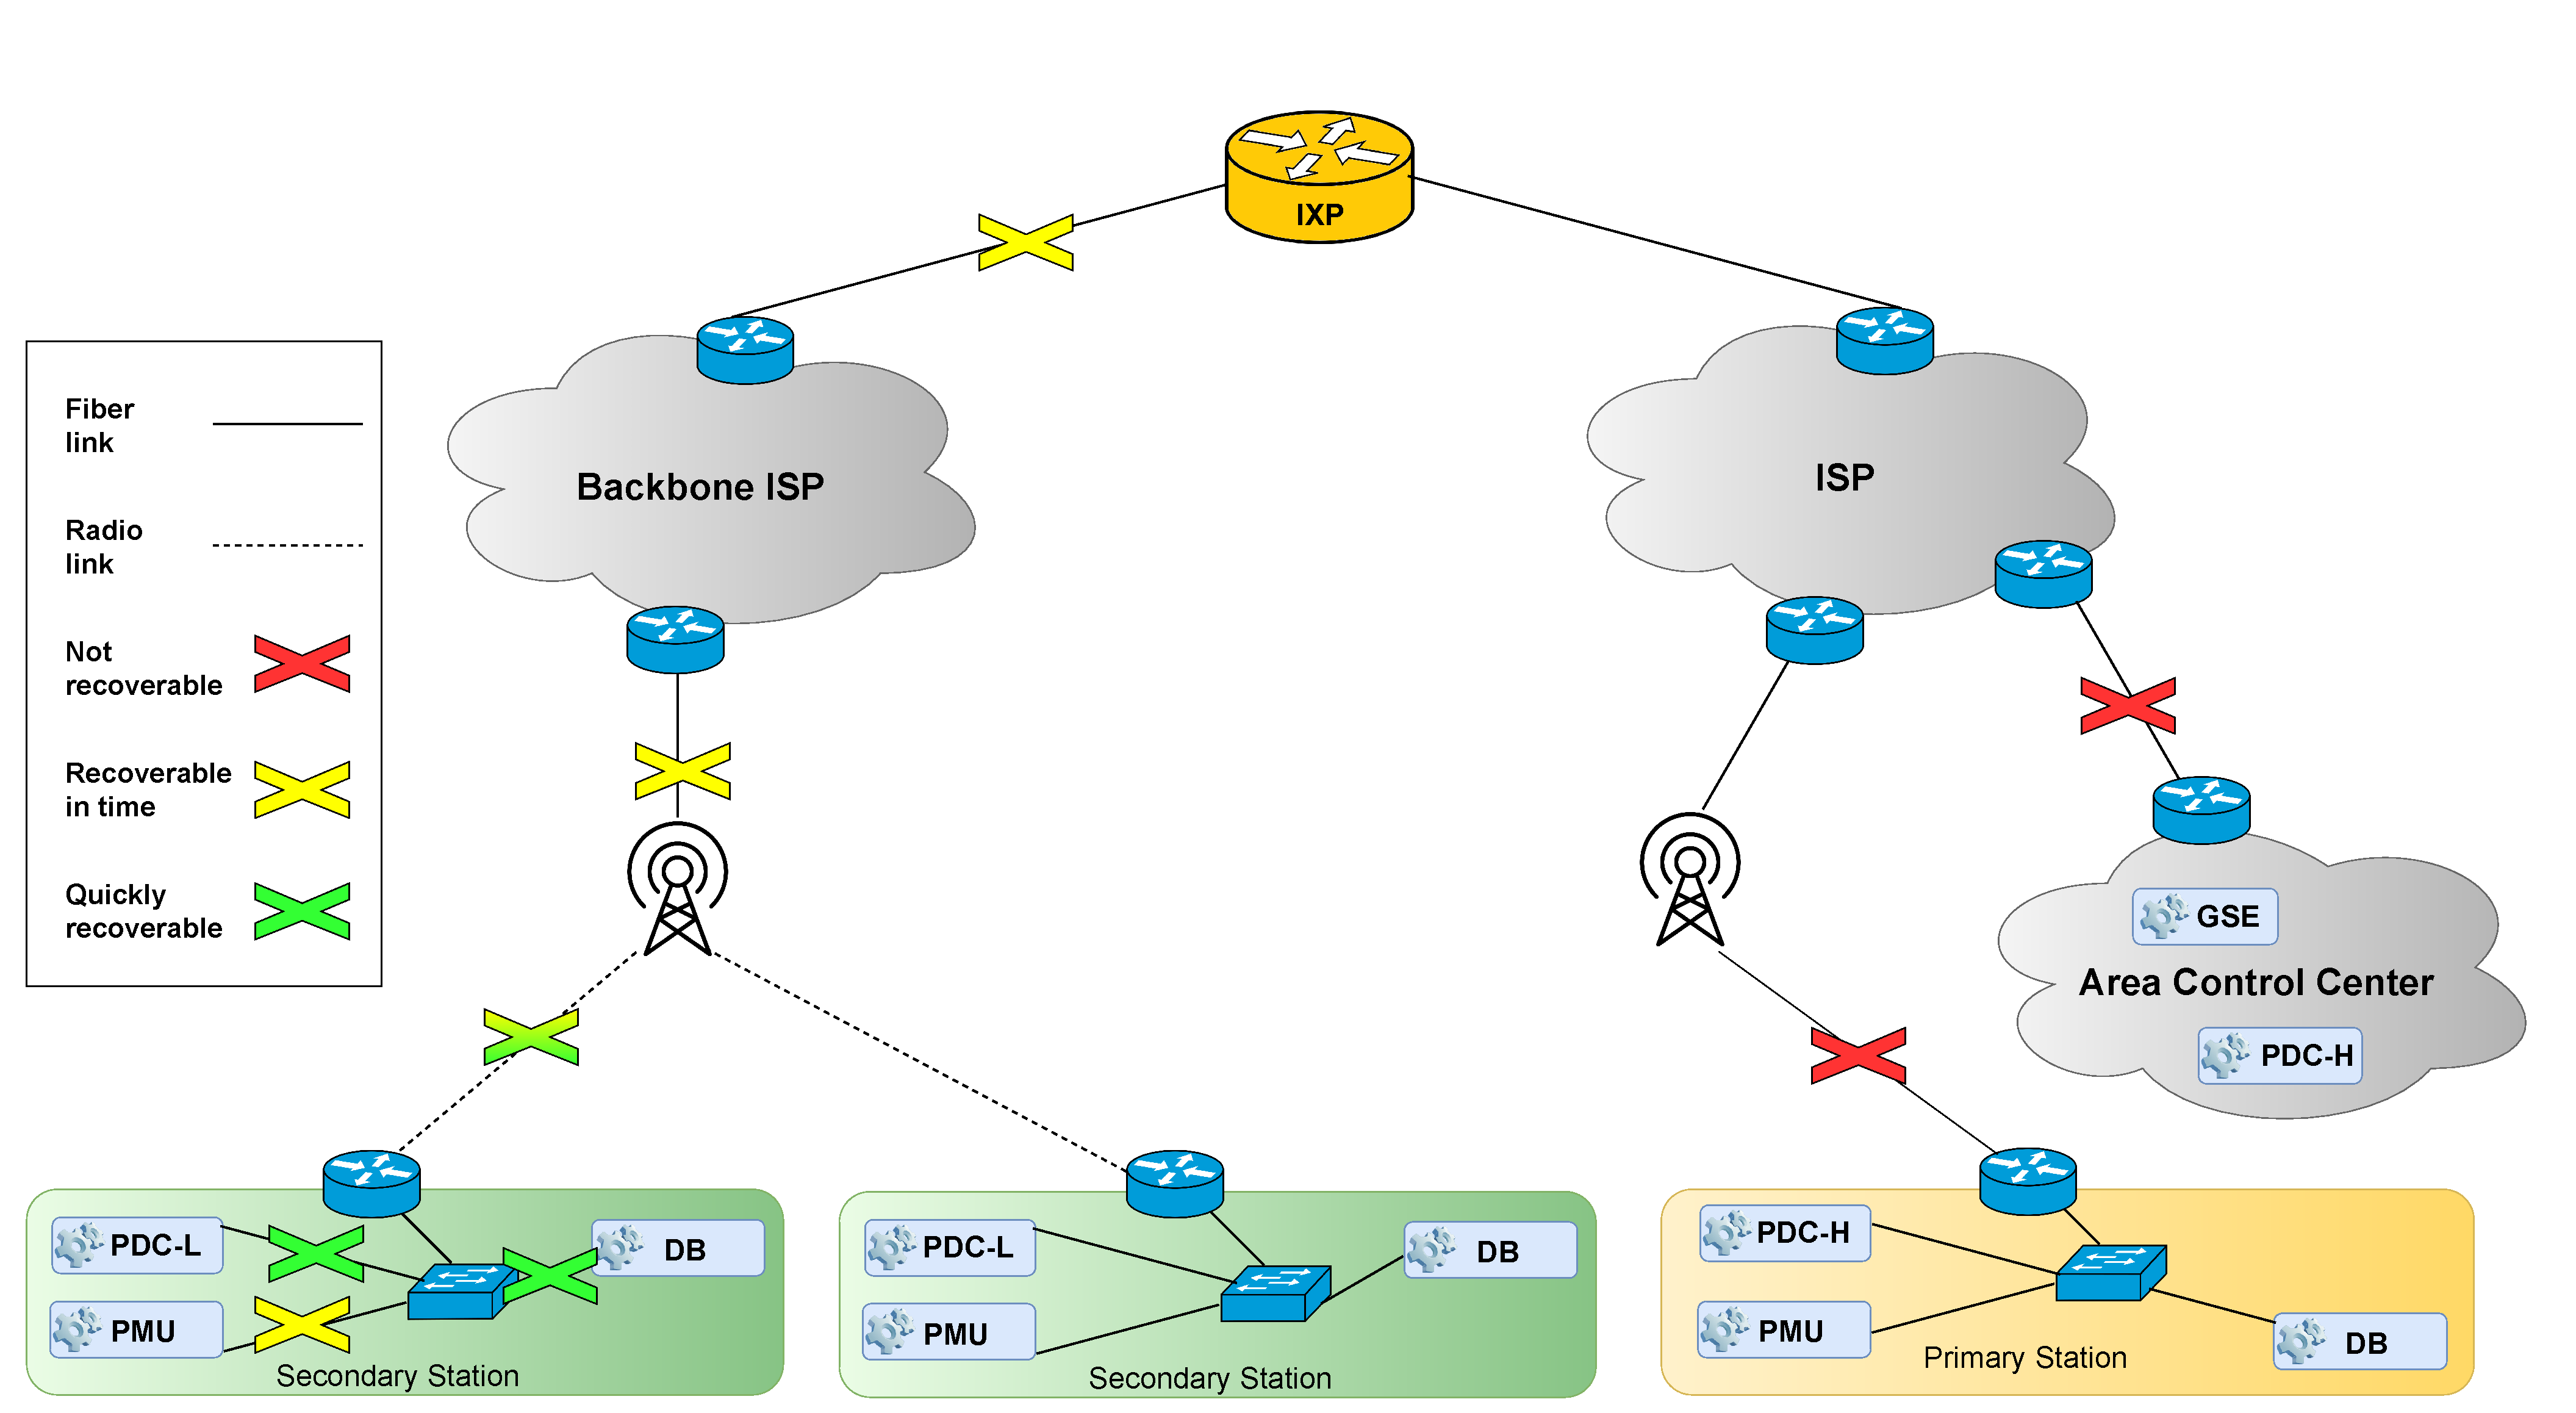
\includegraphics[scale=0.20]{Pictures/failures2}
\caption{Possible failures in multi-level logical domains implementation.}\label{fig:failures2}
\end{figure}

However, this benefit is balanced by a decrease in overall resilience, because in addition to the critical point represented by the Area Control Center, all primary stations that manage a subnetwork of secondary stations also become critical points. This is because a failure or disconnection of the primary station results in the loss of deployment for low-level applications, which is not a feature supported by Liqo technology, thus necessitating a system reset upon reconnection.

Comparing the risks arising from the failure of one component with those that an extended local solution encompassed, as shown in Table ~\ref{t:7}, it can be noted that many have decreased, as there is no longer the possibility of the network remaining unobservable. The risks related to PMU failures have remained the same, as it cannot be rescheduled to another node.

\begin{table}[t]              
\centering 
\begin{tabularx}{\textwidth}{|l|c|X|}
\hline
\textbf{Component Failure} & \textbf{Severity} & \textbf{Cause}\\ 
\hline
\raisebox{-0.75cm}{Single PMU} & \raisebox{-0.75cm}{Low-> Low} & Generally the number of other PMUs guarantees the observability threshold. \\
\hline
\raisebox{-0.75cm}{Multiple PMUs} & \raisebox{-0.75cm}{Low-High-> Low-High} & It depends on whether the number of other PMUs guarantees the observability threshold.\\
\hline
\raisebox{-0.75cm}{Single PDC-l} & \raisebox{-0.75cm}{Moderate-High-> Low-Moderate} & The observability of the network is impaired until the PDC is rescheduled onto another node.\\
\hline
\raisebox{-0.75cm}{Multiple PDCs-l} & \raisebox{-0.75cm}{Moderate-High-> Low-Moderate} & The observability of the network is impaired until the PDCs are rescheduled onto another nodes. \\
\hline
\raisebox{-0.75cm}{Single PDC-h} & \raisebox{-0.75cm}{High-> Moderate}& The observability of the network is impaired until the PDC is rescheduled onto another node. \\
\hline
\end{tabularx}
\caption[Component failures on Multi- level Logical Domains topology overview.]{Component failures on Multi-level Logical Domains topology overview.} \label{t:7}  
\end{table}

This thesis focuses on achieving the highest degree of resilience; therefore, the following chapter will focus on testing the first implementation, as there is no risk of having to redeploy the software components in a subnetwork of secondary substations in the event of a failure of the entire associated primary station cluster.

It is important to note that these two implementations are not mutually exclusive; they can be implemented simultaneously within the same physical network, in cases where different parts of the network require varying degrees of resilience.

\chapter{Domain peering evaluation}

\section{k3s reaction time}
spiegazione e grafici, comparazione con un normale kubernetes, valori minimi

\section{Stream reaction time}
grafici e spiegazione, 

\section{latency}
latenza e grafici, comparazione con latenza senza Liqo

\chapter{conclusion and future work}
conclusioni e lavoro futuro

%%%%%%%%%%%%%%%%%%%%%%%%%%%%%%%%%%%%%%%%%%%%%%%%
%%%%%%%%%%%%%%%%%%%%%%%%%%%%%%%%%%%%%%%%%%%%%%%%


\bibliography{references}



\end{document}

